% folarrow-en.tex: the manual of the folarrow package (English)
% Compile: uplatex folarrow-en && uplatex folarrow-en && dvipdfmx folarrow-en
% (upLaTeX+dvipdfmx, like the Japanese manual, because of the xy-pic examples; in TeX Live 2025
%  and 2026 xy-pic itself fails with LuaLaTeX because of an xypdf error)
\documentclass[dvipdfmx,a4paper]{article}
\usepackage[T1]{fontenc}
\usepackage{lmodern}
\usepackage{textcomp}
\usepackage[margin=25mm]{geometry}
\usepackage{amsmath,amscd}
\usepackage[all]{xy}
\usepackage{tikz-cd}
\usepackage{folarrow}
\usepackage{fancyvrb}
\usepackage{graphicx}
\usepackage{longtable}
\usepackage{url}
\title{The folarrow package\\\large Arrows with three strokes for the projection of a foliated bundle}
\author{Yuwsuke Kieda}
\date{2026-10-10\quad v20261010.0}
\newcommand\pkg[1]{\textsf{#1}}
\newcommand\cs[1]{\texttt{\textbackslash#1}}
\newcommand\file[1]{\texttt{#1}}
\fvset{frame=single,framesep=3mm,fontsize=\small}
\setlength\emergencystretch{3em}
\begin{document}
\maketitle

\noindent A Japanese version of this manual is \file{folarrow-ja.pdf}.

\section{Overview}

When a fiber bundle is drawn as a diagram, its projection is drawn as a vertical arrow.
\[
\begin{CD}
V @>>> E\\
@. @VV{\pi}V\\
@. M
\end{CD}
\]
For a foliated bundle, three slanted strokes are sometimes drawn across the shaft of this arrow.
\[
\begin{CD}
V @>>> E\\
@. @FVV{\pi}V\\
@. M
\end{CD}
\]
The \pkg{folarrow} package makes such arrows available in \pkg{amscd}, \pkg{xy-pic} and
\pkg{tikz-cd} diagrams and in inline math.

The arrows themselves are the usual arrows of each package, and the three strokes are drawn over
the middle of the shaft. The strokes are drawn with \pkg{pict2e} (PGF in \pkg{tikz-cd}), so no
additional fonts are needed for them. The length and the line thickness of the strokes follow the
size of the current math font (font size and math style).

\section{Loading}

\begin{Verbatim}
\usepackage{amscd}      % only the ones you use
\usepackage[all]{xy}
\usepackage{tikz-cd}
\usepackage{folarrow}
\end{Verbatim}
\pkg{amscd}, \pkg{xy-pic} and \pkg{tikz-cd} may be loaded before or after \pkg{folarrow}
(the support for them is set up at \verb|\begin{document}|).

\subsection{Light version: the \texttt{lite} option}\label{sec:lite}
\begin{Verbatim}
\usepackage[lite]{folarrow}
\end{Verbatim}
With \verb|lite|, the package uses no other files (the Lua module, the measured data and the
arrow fonts) and draws all arrows (there is also a separate manual for the light version,
\file{folarrow-lite-en.pdf}). Use it, for example, when you do not want the arrow fonts
embedded in the PDF. Without it (the default), nothing changes.
\begin{itemize}
\item No file other than \file{folarrow.sty} is used, even if installed: not the Lua module
  \file{folarrow.lua}, the measured data \file{folarrow-fonts.def}, the tables of the arrow fonts
  \file{folarrow-glyphs.def} and \file{folarrow-otf.def}, or the arrow fonts and the map file.
\item All arrows, including the inline arrows, are drawn (the fonts of section~\ref{sec:glyphs}
  are not used, and \verb|glyphs| is always false). The result is an arrow with three strokes
  drawn over it, so copying it from the PDF gives the original arrow character (for
  \verb|\foldownarrow|, the pieces of the delimiter).
\item The width of the arrowhead and the line thickness (section~\ref{sec:metrics}) are read
  from the glyph bounding box with Xe\LaTeX{} and an OpenType math font (using
  \verb|\XeTeXglyphbounds|), and estimated from the font dimensions otherwise
  (pdf\LaTeX, up\LaTeX, Lua\LaTeX).
\item Since the measured data is not used, the strokes are placed at the center of the arrow's
  box (without correcting for the offset from the center of the ink), and their ends are always
  butt. For the inline arrows of 10\,pt Computer Modern, \pkg{newtxmath}, \pkg{newpxmath} and
  \pkg{txfonts}, the strokes were off the center by up to 0.3\,pt along the arrow and 0.03\,pt
  across it (at most 0.015\,pt by default). With some fonts the offset is larger, and the width
  and thickness may also differ from the measured values.
\item The workaround of rotating the vertical arrows of Pennstander Math
  (section~\ref{sec:glyphs}) is not applied.
\item \verb|lite| can only be given when loading the package (not with \verb|\folarrowsetup|).
\end{itemize}

\section{amscd}

Add \verb|F| right after the \verb|@| of the usual arrows \verb|@>>>|, \verb|@<<<|, \verb|@VVV|
and \verb|@AAA| to get the strokes. Labels are given in the same way as for the usual arrows.
\begin{Verbatim}
\begin{CD}
V @>>> E @F>f>> E'\\
@VVV @FV{\pi}VV @FAA{\pi'}A\\
M @= M @F<<g< M
\end{CD}
\end{Verbatim}
\[
\begin{CD}
V @>>> E @F>f>> E'\\
@VVV @FV{\pi}VV @FAA{\pi'}A\\
M @= M @F<<g< M
\end{CD}
\]

\section{xy-pic}

The package provides a directional object \verb|fol| to be placed on an arrow. Place it as a
label on the arrow with \verb/|/, as in \verb/\ar[d]|@{fol}/. It is an object of size zero, so
the arrow is not broken. The direction of the strokes follows the direction of the arrow, and it
also works on diagonal arrows.
\begin{Verbatim}
\xymatrix{
V \ar[r] & E \ar[d]|@{fol}^{\folpad{\pi}} \\
         & M }
\end{Verbatim}
\[
\xymatrix{
V \ar[r] & E \ar[d]|@{fol}^{\folpad{\pi}} \\
         & M }
\qquad
\xymatrix{
E \ar[r]|@{fol} & B \ar[d]|@{fol} \ar[dl]|@{fol} \\
M \ar[u]|@{fol} & N \ar[l]|@{fol} }
\]

A label of the arrow is placed at the position of the strokes, so it may overlap them.
Enclose the label in \verb|\folpad|: it adds a margin of half the length of the strokes on
all sides, and the label clears the strokes.
\begin{Verbatim}
\ar[d]|@{fol}^{\folpad{\pi}}
\end{Verbatim}

\section{tikz-cd}

Add \verb|foliated| to the options of the arrow.
\begin{Verbatim}
\begin{tikzcd}
V \arrow[r] & E \arrow[d, foliated, "\pi"] \\
            & M
\end{tikzcd}
\end{Verbatim}
\[
\begin{tikzcd}
V \arrow[r] & E \arrow[d, foliated, "\pi"] \\
            & M
\end{tikzcd}
\qquad
\begin{tikzcd}
E \arrow[r, foliated] & B \arrow[d, foliated] \arrow[dl, foliated] \\
M \arrow[u, foliated] & N \arrow[l, foliated]
\end{tikzcd}
\]
\verb|foliated| uses the \verb|decorations.markings| library (loaded by \pkg{folarrow}).
On arrows with \verb|foliated|, the margin of the labels (\verb|inner sep|) is increased by half
the length of the strokes, so that the labels clear the strokes.

\section{Inline math}

\begin{center}
\renewcommand\arraystretch{1.5}
\begin{tabular}{ll}
\verb|\folrightarrow| & $E\folrightarrow M$\\
\verb|\folleftarrow| & $M\folleftarrow E$\\
\verb|\foldownarrow| & $E\foldownarrow M$\\
\verb|\foluparrow| & $M\foluparrow E$\\
\verb|\xfolrightarrow[below]{above}| & $E\xfolrightarrow{\pi}M$,\ \ $E\xfolrightarrow[\text{proj}]{\pi}M$\\
\verb|\xfolleftarrow[below]{above}| & $M\xfolleftarrow{\pi}E$
\end{tabular}
\end{center}
\begin{itemize}
\item All of them are relations (\verb|\mathrel|) and can be used in subscripts:
  $A_{E\folrightarrow M}$.
\item Base arrows: \verb|\longrightarrow| for \verb|\folrightarrow|, and \verb|\longleftarrow|
  for \verb|\folleftarrow|.
\item \verb|\xfolrightarrow| and \verb|\xfolleftarrow| stretch with the labels above and below,
  like \verb|\xrightarrow| of \pkg{amsmath}, but are never shorter than \verb|\longrightarrow|.
\end{itemize}

\subsection{Fonts for the inline arrows}\label{sec:glyphs}
With the following math fonts, the four arrows \verb|\folrightarrow|, \verb|\folleftarrow|,
\verb|\foldownarrow| and \verb|\foluparrow| are typeset with Type~1 fonts in which each arrow,
including the strokes, is a single glyph.
\begin{center}
\begin{tabular}{lll}
Math font & Symbol font & Arrow font\\\hline
Computer Modern (default) & \file{cmsy5}--\file{cmsy10} & \file{folcm5}--\file{folcm10}\\
Latin Modern (\pkg{lmodern}) & \file{lmsy5}--\file{lmsy10} & \file{follm5}--\file{follm10}\\
\pkg{newtxmath} & \file{ntxsy}, \file{ntxsy7}, \file{ntxsy5} & \file{folntx}, \file{folntx7}, \file{folntx5}\\
\pkg{txfonts} & \file{txsy} & \file{foltx}\\
\pkg{newpxmath} & \file{zplsy} & \file{folzpl}\\
\pkg{pxfonts} & \file{pxsy} & \file{folpx}\\\hline
Computer Modern (bold) & \file{cmbsy5}--\file{cmbsy10} & \file{folcmb5}--\file{folcmb10}\\
Latin Modern (bold) & \file{lmbsy5}, \file{lmbsy7}, \file{lmbsy10} & \file{follmb5}, \file{follmb7}, \file{follmb10}\\
\pkg{newtxmath} (bold) & \file{ntxbsy}, \file{ntxbsy7}, \file{ntxbsy5} & \file{folntxb}, \file{folntxb7}, \file{folntxb5}\\
\pkg{txfonts} (bold) & \file{txbsy} & \file{foltxb}\\
\pkg{newpxmath} (bold) & \file{zplbsy} & \file{folzplb}\\
\pkg{pxfonts} (bold) & \file{pxbsy} & \file{folpxb}
\end{tabular}
\end{center}
\begin{itemize}
\item A glyph is the outline of the minus sign and $\rightarrow$ of the symbol font (combined
  in the same way as \verb|\longrightarrow|) with the outlines of the three strokes added.
  $\leftarrow$ is made from $\leftarrow$ and the minus sign, and $\downarrow$ and $\uparrow$ are
  the glyph of $\rightarrow$ rotated, centered on the math axis. The length, spacing, slant,
  thickness and ends of the strokes are computed from the outline of the original glyph by the
  same rules as the default when drawing. The center of the strokes is at the center of the
  arrow's ink.
\item The result is a single character of a font, so copying it from the PDF gives
  U+2192, U+2190, U+2193 and U+2191.
\item The font is loaded at the same size as the symbol font, so in subscripts or with
  \verb|\large| the glyph corresponds to the symbol font of that size.
\item When a shape key (section~\ref{sec:shape}) is not at its default, with
  \verb|glyphs=false|, or with a math font in neither the table above nor the list of OpenType
  math fonts below, the strokes are drawn over the arrow as before. Then the base of
  $\downarrow$ and $\uparrow$ is a delimiter 1.25 times the quad of the symbol font high.
\item The stretchable arrows (\verb|\xfolrightarrow| etc.) and the arrows of diagrams change
  their length, so they are always drawn.
\end{itemize}
\paragraph{OpenType math fonts}
With Lua\LaTeX{} and Xe\LaTeX{} and \pkg{unicode-math}, the arrows are typeset with OTF fonts
(\file{folu-\textit{code}.otf}) for the following 49 fonts.
\begin{quote}\small
Latin Modern Math, New Computer Modern Math (Regular, Book, Bold), New Computer Modern Sans Math,
STIX Two Math, STIX Math, XITS Math (Regular, Bold), \TeX{} Gyre Termes, Pagella, Bonum, Schola and DejaVu Math,
Libertinus Math, Fira Math, Asana Math, Erewhon Math (Regular, Bold),
KpMath (Regular, Light, Semibold, Bold, Sans, SansBold), GFS Neohellenic Math, IBM Plex Math,
Arsenal Math (Sans, SansBold), Concrete Math (Regular, Bold), Euler Math, Garamond Math,
Lete Sans Math (Regular, Bold), Luciole Math (Regular, Bold), Old Standard Math,
XCharter Math (Regular, Bold), Pennstander Math (nine weights from Thin to Black)
\end{quote}
\begin{itemize}
\item XITS Math Bold has no U+27F6 and U+27F5, so, like \verb|\relbar\joinrel\rightarrow| in
  \LaTeX, an outline of the minus sign and $\rightarrow$ ($\leftarrow$ and the minus sign)
  overlapped by 3/18\,em is used as the long arrow. When drawing, too, arrows are made with
  \verb|\relbar\joinrel\rightarrow| etc.\ if the font has no U+27F6 or U+27F5.
\item A glyph is the outline of U+27F6 (\verb|\longrightarrow|) or U+27F5 (\verb|\longleftarrow|)
  of the original font with the outlines of the strokes added. $\downarrow$ and $\uparrow$ are
  U+27F6 rotated, centered on AxisHeight of the MATH table. The thickness and height of the shaft
  are measured by cutting the outline of the arrow vertically, and the shape of the tail is also
  determined from the outline (round if the distance from the end to where the shaft reaches its
  full width is at least 0.35 times the thickness).
\item When the original font has script glyphs (\texttt{ssty}) for the arrows (Erewhon Math,
  Concrete Math, Lete Sans Math, Luciole Math, XCharter Math (Regular only for each), Euler Math,
  Pennstander Math), glyphs are made from each of them, the font gets the same \texttt{ssty}
  feature, and it is loaded with the same options as the original font (\verb|+ssty=0| etc.).
\item The original font is identified by whether the font name part of \verb|\fontname| (a file
  name or a font name) matches the file name, PostScript name, full name or family name of an
  original font.
\item The characters are at their Unicode positions (U+2192, U+2190, U+2193, U+2191), so as text
  they are $\rightarrow\leftarrow\downarrow\uparrow$.
\item In Pennstander Math, the axis of the shaft piece and that of the head piece of the
  extensible $\downarrow$ (GlyphAssembly of the MATH table) are misaligned, and a large delimiter
  $\downarrow$ is broken ($\uparrow$ has no extensible data; this happens without \pkg{folarrow}
  too). So, for the nine fonts of this family, the base of the drawn vertical arrows
  (\verb|\foldownarrow| and \verb|\foluparrow| with \verb|glyphs=false| etc., and \verb|@FVVV| and
  \verb|@FAAA| of \pkg{amscd}) is not a delimiter but a horizontal arrow
  (\verb|\longrightarrow| inline, a stretchable arrow as long as \verb|\Big| for \pkg{amscd})
  rotated by 90\textdegree. The center of the ink is taken from the bounding box of the glyph
  before rotation and is aligned to the math axis. The affected fonts are determined from their
  extensible pieces and listed in \file{folarrow-otf.def}. The broken vertical arrows where
  \pkg{folarrow} commands are not used (usual \verb|@VVV| and \verb|@AAA| of \pkg{amscd},
  \verb|\Big\downarrow|, etc.)\ are a problem of the font and are not supported.
\item U+27F6 and U+27F5 of XCharter Math Bold have ink longer than their advance width (1000),
  up to 1524, and overlap the next character (a problem of the font). In the OTF, a glyph whose
  ink exceeds its advance width gets the advance width of the right edge of the ink plus the left
  side bearing (1580, as in Regular). When drawing, the original width is kept, so they overlap.
\item The OTF fonts were made from the original fonts. They keep the licenses of the original
  fonts, the SIL Open Font License 1.1 or the GUST Font License. Their file names and font names
  (\texttt{FolArrowU-\textit{code}}) do not contain the names (Reserved Font Names) of the
  original fonts. There are none for fonts that may not be redistributed, such as Minion Math
  (the arrows are drawn as before).
\end{itemize}

The map file of the Type~1 fonts, \file{folarrow.map}, is loaded by the package with
pdf\LaTeX{} and Lua\LaTeX; with dvipdfmx and xdvipdfmx the package issues
\verb|\special{pdf:mapfile folarrow.map}| on the first page.
For dvips, enable \file{folarrow.map} with \file{updmap}.

The Type~1 arrow fonts were made from the original symbol fonts and keep their licenses:
SIL Open Font License 1.1 for those from Computer Modern (named \file{folcm} and
\texttt{FolArrow-CM} to avoid the Reserved Font Names), GUST Font License for those from
Latin Modern, and GPL (with the font exception) for those from \pkg{txfonts}, \pkg{pxfonts},
\pkg{newtx} and \pkg{newpx}.

\subsection{Bold}\label{sec:bold}
When math is made bold with \verb|\boldmath| (\verb|\mathversion{bold}|) or \verb|\bm| of
\pkg{bm}, the arrows are typeset with the bold symbol fonts, and the strokes follow them.
\begin{itemize}
\item Type~1 math fonts (Computer Modern, Latin Modern, \pkg{newtx}, \pkg{txfonts}, \pkg{newpx},
  \pkg{pxfonts}): the inline arrows are typeset with the arrow fonts made from the bold symbol
  fonts (the bold rows of the table above), and the vertical arrows are bold too. The length and
  thickness of the strokes of the stretchable arrows and the arrows of diagrams are taken from
  the measured data of the bold symbol fonts.
\item The vertical arrows of \pkg{amscd} are large delimiters, so they are bold if the font of
  large delimiters has a bold version (\pkg{newtx}, \pkg{txfonts}, \pkg{newpx}, \pkg{pxfonts}).
  \file{cmex10} and \file{lmex10} of Computer Modern and Latin Modern have no bold version, so
  the vertical arrows do not get thicker in bold (as with the usual \verb|\Big\downarrow| of
  \LaTeX). The strokes follow that arrow.
\item \pkg{unicode-math}: specify the bold math font with \verb|version=bold|, as in
\begin{Verbatim}
\setmathfont{NewCMMath-Bold.otf}[version=bold]
\end{Verbatim}
  and \verb|\boldmath| switches to it.
  The inline arrows are typeset with the OTF font for the bold font (Bold etc.\ in the list of
  section~\ref{sec:glyphs}), and the strokes of the drawn arrows are computed from the glyphs of
  the bold font. With fonts that have no extensible data for $\downarrow$, such as KpMath Bold
  and Erewhon Math Bold, the vertical arrows of \pkg{amscd} remain short glyphs (like the usual
  \verb|@VVV|).
\item In New Computer Modern Math Bold, the dimensions of the extensible pieces of $\downarrow$
  are broken, and Xe\LaTeX{} does not stop when it tries to build a large delimiter $\downarrow$
  (\verb|\Big\downarrow| etc.; this happens without \pkg{folarrow} too). So, only with
  Xe\LaTeX, the drawn vertical arrows (\verb|@FVVV| and \verb|@FAAA| of \pkg{amscd} etc.)\ are
  built from a rotated horizontal arrow, as for Pennstander Math.
\item The light version (\verb|lite|) does not use the measured data, so the length and
  thickness of the strokes in bold are estimates.
\end{itemize}
Measuring the bold versions of Computer Modern, Latin Modern, \pkg{newtx}, \pkg{txfonts},
\pkg{newpx} and \pkg{pxfonts} typeset with \verb|\boldmath|, the ratio of the computed to the
measured width of the arrowhead and thickness of the shaft was 0.99--1.01 for all sizes and
styles with pdf\LaTeX{} and up\LaTeX. The offset of the strokes from the center was at most
0.07\,pt, except for the stretchable arrows (up to 0.17\,pt for bold \pkg{pxfonts}; the limit of
\verb|\cleaders| in section~\ref{sec:metrics}).

\section{Adjusting the strokes}\label{sec:shape}

Use package options or \verb|\folarrowsetup|. \verb|\folarrowsetup| inside a group affects only
that group.
\begin{Verbatim}
\usepackage[gap=0.45]{folarrow}
\folarrowsetup{span=1.2, thickness=0.5pt}
\end{Verbatim}
\begin{center}\small
\begin{tabular}{lll}
Key & Default & Meaning\\\hline
\verb|span| & 1.0 & length of the strokes (ratio to the arrowhead width; $>0$, $\le 10$)\\
\verb|lean| & 0.25 & slant (offset along the arrow relative to the length; $-5$ to 5)\\
\verb|gap| & 0.35 & spacing of the strokes (ratio to the arrowhead width; 0 to 10)\\
\verb|shift| & 0 & shift from the middle toward the tail (ratio to the arrowhead width; $-10$ to 10)\\
\verb|thickness| & (empty) & line thickness (a length $\ge 0$); if empty, the shaft thickness (section~\ref{sec:metrics})\\
\verb|glyphs| & true & use the arrow fonts for the inline arrows (section~\ref{sec:glyphs})\\
\verb|lite| & false & light version (only when loading; section~\ref{sec:lite})
\end{tabular}
\end{center}
\par\noindent\begin{minipage}{\linewidth}
\paragraph{Example}
The following document uses \verb|\folarrowsetup|. It can be copied as it is, from
\verb|\documentclass| to \verb|\end{document}|, and compiled
(\file{full-examples/ex-setup-en.tex}; the result is that example actually typeset).
\VerbatimInput{full-examples/ex-setup-en.tex}
\par\noindent Result:\par
\begin{center}\fbox{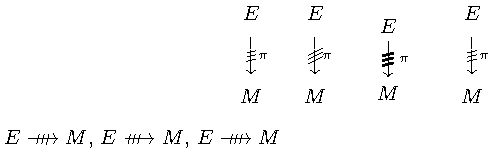
\includegraphics{full-examples/ex-setup-en-out.pdf}}\end{center}
\end{minipage}\par\medskip
\verb|\folarrowsetup{gap=0.45}| in the preamble affects the whole document. \verb|\folarrowsetup|
used inside a group (\verb|{| and \verb|}|) affects only that group, and the setting of the whole
document is restored after the group. The diagrams are, from left to right: the setting of the
whole document (\verb|gap=0.45|); in addition \verb|span=1.5, lean=0.5|;
\verb|thickness=0.8pt| (\pkg{tikz-cd}); back to the setting of the whole document. The inline
arrows are, from left to right: the setting of the whole document; in addition \verb|shift=0.5|
(the strokes are moved toward the tail of the arrow); back to the setting of the whole document.
Since the shape keys are not at their defaults, the inline arrows of this example are not
typeset with the arrow fonts of section~\ref{sec:glyphs} but drawn with the strokes over the
arrow.

How the width of the arrowhead, which is the reference for the size of the strokes, and the line
thickness are determined is described in section~\ref{sec:metrics}. In \pkg{tikz-cd}, if
\verb|thickness| is empty, the strokes are drawn as thick as the shaft of the arrow.

Of the two directions ``$\pm\text{lean}\times\text{direction of the arrow}+\text{normal}$'', the
strokes take the one that rises to the right. On horizontal arrows they are upright ``///'', and
on vertical arrows they are three nearly horizontal strokes rising to the right.

\section{Width of the arrowhead and line thickness}\label{sec:metrics}

The length and spacing of the strokes are based on the width of the arrowhead, and the line
thickness on the thickness of the shaft. These differ greatly among fonts (even at 10\,pt, the
arrowhead width ranges from 2.4\,pt to 5.6\,pt) and often cannot be obtained correctly from the
font metrics (TFM or \verb|\fontdimen|). So they are determined for the arrow font actually used,
in the following order.
\begin{enumerate}
\item \textbf{Lua\LaTeX{} with an OpenType math font}: the bounding box of the glyph in the
  arrow's box is read directly from the font and gives the arrowhead width. The line thickness is
  the height of the minus sign (U+2212) of the same font. Script glyphs (OpenType ssty) used at
  script sizes and the large glyphs of \verb|\Big| are also read (\file{folarrow.lua}).
\item \textbf{Xe\LaTeX{} with an OpenType math font}: the bounding box of the glyph is read with
  \verb|\XeTeXglyphbounds|. Script glyphs and the large glyphs of \verb|\Big| cannot be read, so
  the values of the base glyph are used.
\item \textbf{Type~1 math fonts} (pdf\LaTeX, up\LaTeX, Lua\LaTeX): the measured data
  (\file{folarrow-fonts.def}) is looked up. The font that has the arrow characters is found from
  the math code of \verb|\rightarrow| and the delimiter code of \verb|\downarrow| (some packages,
  such as \pkg{drm} and \pkg{euler}, take the arrows from fonts other than the symbol font).
  The data has, for each font name (the base part of \verb|\fontname|), the ratios of the
  arrowhead width and the shaft thickness to the quad. Fonts whose shapes differ with optical
  size, such as cmsy7 and cmsy10, have entries under their own names.
\item \textbf{Otherwise}: the values are estimated from the height of the box of
  \verb|\rightarrow|, the height of the math axis and the rule thickness of the math extension
  font. The ratios to the quad are limited to avoid extreme values.
\end{enumerate}
For OpenType fonts whose minus sign is not as thick as the shaft of the arrow (Asana Math,
GFS Neohellenic Math, the \verb|\Big| glyphs of Minion Math and of KpMath), a correction
measured from the fonts is applied.

\subsection{Position of the strokes}

The strokes are placed at the center of the arrow's ink (on the shaft, at the middle of the
arrow's length). The center of the arrow's box and the center of its ink often differ
(for the base of \verb|\foldownarrow| and \verb|\foluparrow| and for \verb|\longrightarrow|,
by about 0.1--0.7\,pt toward the head, and with some fonts by 0.1--0.3\,pt across the shaft).
A left arrow is not necessarily a mirrored right arrow, so its offsets differ from those of the
right arrow. So, for each of eight kinds of arrows (\verb|\longrightarrow|, \verb|\longleftarrow|,
the right and left stretchable arrows, the down and up arrows of \verb|\Big|, and the bases of
\verb|\foldownarrow| and \verb|\foluparrow|), the measured data has the difference between the
center of the box and the center of the ink in the two directions along and across the arrow,
and the strokes are moved by that amount. With Lua\LaTeX{} and Xe\LaTeX, the height of the
strokes on horizontal arrows is the vertical center of the arrowhead taken from the glyph's
bounding box.

The base of \verb|\foldownarrow| and \verb|\foluparrow| is a delimiter 1.25 times the quad of the
symbol font high. The width of the empty delimiter added by \verb|\right.|
(\verb|\nulldelimiterspace|) is set to 0, and \verb|\delimiterfactor| is set to 1000 and
\verb|\delimitershortfall| to 0, so that the choice of the delimiter glyph does not depend on the
font size or the text font.

On stretchable arrows (horizontal arrows of \pkg{amscd}, \verb|\xfolrightarrow|), the
distribution of the \verb|\cleaders| that fill the shaft changes with the length of the arrow,
so with some fonts an offset of about 0.1\,pt remains (0.14\,pt with STIX, 0.17\,pt with bold
\pkg{pxfonts}).

In the arrow fonts of section~\ref{sec:glyphs}, the strokes are placed at the center of the ink
computed from the outline of the glyph. Measuring the arrows in four directions of 10\,pt
Computer Modern, \pkg{newtxmath}, \pkg{newpxmath} and \pkg{txfonts} in 2400\,dpi images, the
offset from the center was at most 0.015\,pt (half a pixel) both along and across the arrow.
For the OTF fonts for OpenType math fonts, the 48 fonts other than XITS Math Bold were typeset
with Lua\LaTeX{} and Xe\LaTeX{} and the arrows in four directions measured in the same way. The
offset across the arrow was at most 0.03\,pt for all fonts, and along the arrow at most
0.03\,pt except for the nine weights of Pennstander Math and Luciole Math Bold. These ten fonts
have long barbs reaching back from the arrowhead, which enter the range where the measurement
looks for the strokes (25--75\% of the arrow's length), so they cannot be measured from images.
So, for the glyphs of all fonts, the original arrow was subtracted from the glyph to extract the
strokes, and their center was compared in outline coordinates: the offset was at most
0.0002\,em (the rounding of coordinates to integers).

In the heavy weights of Pennstander Math (Bold and heavier), the shaft is about as thick as the
spacing of the strokes, so the strokes appear joined (this follows from the rules of the shape).
With Lua\LaTeX, the extensible $\uparrow$ of Luciole Math gives the error ``Extensible recipe has
no fixed parts'' (a problem of the font; it happens without \pkg{folarrow} too). The glyphs of the
OTF fonts do not use this delimiter, so they are not affected, but a drawn \verb|\foluparrow|
(with \verb|glyphs=false| etc., including the light version \verb|lite|, which always draws)
gives this error.

\subsection{Ends of the strokes}

The ends of the strokes follow the shape of the arrow's tail (the end of the shaft): round ends
for arrows with a round tail, butt ends otherwise. A round end extends half the line thickness
beyond the end, so round strokes are drawn shorter by that amount to keep the same visual length.
\begin{itemize}
\item \pkg{amscd}, inline math: the measured data has the shape of the tail for each way the
  arrow is actually built (\verb|\longrightarrow|, stretchable arrows, \verb|\Big\downarrow|, the
  base of \verb|\foldownarrow|). For example, in Computer Modern the horizontal arrows have a
  round tail (the end of \verb|\relbar| is round) and \verb|\Big\downarrow| has a flat top, so the
  strokes have round ends on horizontal arrows and butt ends on vertical arrows. OpenType math
  fonts are looked up in a table by font name (round for Latin Modern Math and New Computer
  Modern Math, butt for the others). Fonts not in the table get butt ends.
\item \pkg{xy-pic}: the lines of \pkg{xy-pic} have round ends, so the strokes have round ends.
\item \pkg{tikz-cd}: the line cap setting of the arrow (\verb|line cap|) is used as it is.
  The default of \pkg{tikz-cd} is butt.
\end{itemize}

\subsection{Verification}

For all fonts (68) of ``Fonts with Math Support'' of The \LaTeX{} Font Catalogue
(\url{https://tug.org/FontCatalogue/mathfonts.html}), OpenType math fonts (Latin Modern Math,
New Computer Modern Math, STIX Two Math, \TeX{} Gyre Termes, Pagella, Bonum, Schola and DejaVu Math,
Libertinus Math, Fira Math, XITS Math, Asana Math, Erewhon Math, KpMath, GFS Neohellenic Math,
Minion Math), and the bold versions (\verb|\boldmath|) of Computer Modern, Latin Modern,
\pkg{newtx}, \pkg{txfonts}, \pkg{newpx} and \pkg{pxfonts}, the arrows were actually typeset and
rendered at 2400\,dpi, and the extent of the ink was measured and compared with the values
computed by \pkg{folarrow}. The sizes were 10\,pt, 10.95\,pt and 12\,pt, the styles text, script
and scriptscript, and the vertical arrows \verb|\Big\downarrow| and the base of
\verb|\foldownarrow|. Type~1 fonts were typeset with pdf\LaTeX{} and up\LaTeX, OpenType fonts
with Lua\LaTeX{} and Xe\LaTeX.

The table below gives the largest difference (\%) between the computed and the measured values;
values above 3\% are in bold. The ``Center'' column is the largest offset (pt) between the
center of the strokes and the center of the arrow's ink (along and across the arrow, over all
sizes of the eight kinds of arrows); values above 0.05\,pt are in bold. The ``Ends'' column is
``ok'' if the measured shape of the arrow's tail (round or flat) and the shape of the stroke
ends chosen by \pkg{folarrow} agree for all four kinds of arrows (\verb|\longrightarrow|,
stretchable arrows, \verb|\Big\downarrow|, the base of \verb|\foldownarrow|).
Only the following exceed 3\%.
\begin{itemize}
\item \textbf{PK fonts} (\pkg{boisik}, Computer Concrete, \pkg{drm}): bitmap fonts made with
  METAFONT, whose pixel steps (0.12\,pt at 600\,dpi) become errors in the dimensions as they are.
  This is a property of the fonts themselves.
\item \textbf{Script glyphs} (STIX Two Math and Erewhon Math with Xe\LaTeX): Xe\TeX{} cannot read
  script glyphs, so the values are off by up to 20\% at script sizes. With Lua\LaTeX{} they are
  correct.
\item \textbf{Not installed}: URW Garamond (\pkg{mathdesign}) and \pkg{garamondx} are non-free
  fonts that are not in the environment used for the verification (\TeX{} Live 2026), so they
  were not checked.
\end{itemize}
The table and the data were made from the results of actually typesetting and measuring the
arrows.

{\small% folarrow-verify-en.tex: verification table made from the results of typesetting and measuring the arrows (generated; do not edit)
\begin{longtable}{@{}lcrrrrrcl@{}}
Font (setting) & Engine & \multicolumn{2}{c}{Horizontal} & \multicolumn{2}{c}{Vertical} & Center & Ends & Note\\
 & & width & thick. & width & thick. & pt & & \\\hline\endhead
\texttt{antykwatorunska} & pdf & 1 & 0 & 0 & 0 & 0.05 & ok & \\
\texttt{antykwatorunska} & up & 1 & 0 & 0 & 0 & \textbf{0.06} & ok & \\
\texttt{antykwatorunskacondensed} & pdf & 1 & 0 & 0 & 0 & 0.02 & ok & \\
\texttt{antykwatorunskacondensed} & up & 1 & 0 & 0 & 0 & 0.02 & ok & \\
\texttt{antykwatorunskalight} & pdf & 1 & 0 & 0 & 0 & \textbf{0.07} & ok & \\
\texttt{antykwatorunskalight} & up & 1 & 0 & 0 & 0 & \textbf{0.07} & ok & \\
\texttt{antykwatorunskalightcondensed} & pdf & 1 & 0 & 0 & 0 & 0.02 & ok & \\
\texttt{antykwatorunskalightcondensed} & up & 1 & 0 & 0 & 0 & 0.03 & ok & \\
\texttt{arev} & pdf & 1 & 0 & 0 & 0 & 0.03 & ok & \\
\texttt{arev} & up & 1 & 0 & 0 & 0 & 0.05 & ok & \\
\texttt{Asana-Math.otf} & Lua & 1 & 0 & 1 & 0 & 0.03 & ok & \\
\texttt{Asana-Math.otf} & Xe & 1 & 0 & 1 & 0 & 0.03 & ok & \\
\texttt{asanamath} & Lua & 1 & 0 & 1 & 0 & 0.03 & ok & \\
\texttt{baskervaldx} & pdf & 0 & 0 & 0 & 0 & 0.02 & ok & \\
\texttt{baskervaldx} & up & 0 & 0 & 0 & 0 & 0.02 & ok & \\
\texttt{baskervillef} & pdf & 0 & 0 & 0 & 0 & 0.02 & ok & \\
\texttt{baskervillef} & up & 0 & 0 & 0 & 0 & 0.02 & ok & \\
\texttt{boisik} & pdf & \textbf{12} & \textbf{27} & 0 & 0 & \textbf{0.20} & ok & PK font\\
\texttt{boisik} & up & \textbf{12} & \textbf{27} & 0 & 0 & \textbf{0.29} & ok & PK font\\
\texttt{charterbt} & pdf & 2 & 0 & 0 & 0 & 0.02 & ok & \\
\texttt{charterbt} & up & 2 & 0 & 0 & 0 & \textbf{0.05} & ok & \\
\texttt{cochineal} & pdf & 0 & 0 & 0 & 0 & 0.02 & ok & \\
\texttt{computerconcrete} & pdf & 1 & \textbf{10} & 0 & 0 & 0.05 & ok & PK font\\
\texttt{computerconcrete} & up & 1 & \textbf{10} & 0 & 0 & \textbf{0.14} & ok & PK font\\
\texttt{computerconcreteeuler} & pdf & 0 & 0 & 0 & 0 & 0.03 & ok & \\
\texttt{computerconcreteeuler} & up & 0 & 0 & 0 & 0 & 0.04 & ok & \\
\texttt{computermodern} & pdf & 0 & 0 & 0 & 0 & 0.03 & ok & \\
\texttt{computermodern} & up & 0 & 0 & 0 & 0 & 0.04 & ok & \\
\texttt{computermodern-bold} & pdf & 0 & 0 & 0 & 0 & 0.03 & ok & \\
\texttt{computermodern-bold} & up & 0 & 0 & 0 & 0 & 0.03 & ok & \\
\texttt{computermodernbright} & pdf & 0 & 0 & 0 & 0 & 0.02 & ok & \\
\texttt{computermodernbright} & up & 0 & 0 & 0 & 0 & 0.03 & ok & \\
\texttt{domitian} & pdf & 1 & 0 & 0 & 0 & 0.02 & ok & \\
\texttt{domitian} & up & 1 & 0 & 0 & 0 & 0.04 & ok & \\
\texttt{drm} & pdf & \textbf{3} & \textbf{13} & 0 & \textbf{6} & \textbf{0.47} & ok & PK font\\
\texttt{drm} & up & 0 & \textbf{5} & 0 & \textbf{6} & \textbf{0.47} & ok & PK font\\
\texttt{ebgaramond} & pdf & 0 & 0 & 0 & 0 & 0.02 & ok & \\
\texttt{ebgaramond} & up & 0 & 0 & 0 & 0 & 0.02 & ok & \\
\texttt{erewhon} & pdf & 0 & 0 & 0 & 0 & 0.02 & ok & \\
\texttt{erewhon} & up & 0 & 0 & 0 & 0 & 0.02 & ok & \\
\texttt{erewhon-math} & Lua & 2 & 0 & 1 & 0 & 0.03 & ok & \\
\texttt{Erewhon-Math.otf} & Lua & 2 & 0 & 1 & 0 & 0.03 & ok & \\
\texttt{Erewhon-Math.otf} & Xe & \textbf{6} & \textbf{18} & 1 & 0 & 0.03 & ok & script glyphs\\
\texttt{eulervm} & pdf & 0 & 0 & 0 & 0 & 0.02 & ok & \\
\texttt{europeancomputerconcrete} & pdf & 1 & \textbf{10} & 0 & 0 & 0.05 & ok & PK font\\
\texttt{europeancomputerconcrete} & up & 1 & \textbf{10} & 0 & 0 & \textbf{0.14} & ok & PK font\\
\texttt{europeancomputerconcreteeuler} & pdf & 0 & 0 & 0 & 0 & 0.03 & ok & \\
\texttt{europeancomputerconcreteeuler} & up & 0 & 0 & 0 & 0 & 0.04 & ok & \\
\texttt{europeancomputermodern} & pdf & 0 & 0 & 0 & 0 & 0.03 & ok & \\
\texttt{europeancomputermodern} & up & 0 & 0 & 0 & 0 & 0.04 & ok & \\
\texttt{europeancomputermodernbright} & pdf & 0 & 0 & 0 & 0 & 0.02 & ok & \\
\texttt{europeancomputermodernbright} & up & 0 & 0 & 0 & 0 & 0.03 & ok & \\
\texttt{Fira Math} & Lua & 2 & 0 & 1 & 0 & 0.02 & ok & \\
\texttt{FiraMath-Regular.otf} & Lua & 2 & 0 & 1 & 0 & 0.02 & ok & \\
\texttt{FiraMath-Regular.otf} & Xe & 2 & 0 & 1 & 0 & 0.02 & ok & \\
\texttt{firasansmath} & Lua & 2 & 0 & 1 & 0 & 0.02 & ok & \\
\texttt{firasansnewtxsf} & pdf & 0 & 0 & 0 & 0 & 0.02 & ok & \\
\texttt{firasansnewtxsf} & up & 0 & 0 & 0 & 0 & 0.02 & ok & \\
\texttt{fourier-only} & pdf & 1 & 0 & 0 & 0 & 0.04 & ok & \\
\texttt{garamond} & pdf & -- & -- & -- & -- & -- & -- & not installed\\
\texttt{garamond} & up & -- & -- & -- & -- & -- & ok & not installed\\
\texttt{garamondexpertmathdesign} & pdf & -- & -- & -- & -- & -- & -- & not installed\\
\texttt{garamondexpertmathdesign} & up & -- & -- & -- & -- & -- & -- & not installed\\
\texttt{garamondexpertnewtxmath} & pdf & -- & -- & -- & -- & -- & -- & not installed\\
\texttt{garamondexpertnewtxmath} & up & -- & -- & -- & -- & -- & -- & not installed\\
\texttt{gfsartemisia} & pdf & 1 & 0 & 0 & 0 & 0.03 & ok & \\
\texttt{gfsartemisia} & up & 1 & 0 & 0 & 0 & 0.02 & ok & \\
\texttt{gfsartemisiaeulermath} & pdf & 0 & 0 & 0 & 0 & 0.03 & ok & \\
\texttt{gfsartemisiaeulermath} & up & 0 & 0 & 0 & 0 & 0.04 & ok & \\
\texttt{gfsneohellenic} & pdf & 0 & 0 & 0 & 0 & 0.03 & ok & \\
\texttt{gfsneohellenic} & up & 0 & 0 & 0 & 0 & 0.04 & ok & \\
\texttt{gfsneohellenicmath} & Lua & 1 & 2 & 1 & 0 & 0.04 & ok & \\
\texttt{GFSNeohellenicMath.otf} & Lua & 1 & 2 & 1 & 0 & 0.03 & ok & \\
\texttt{GFSNeohellenicMath.otf} & Xe & 1 & 2 & 1 & 0 & 0.03 & ok & \\
\texttt{heuristica} & pdf & 0 & 0 & 0 & 0 & 0.02 & ok & \\
\texttt{heuristica} & up & 0 & 0 & 0 & 0 & 0.02 & ok & \\
\texttt{iwona} & pdf & 1 & 0 & 0 & 0 & 0.03 & ok & \\
\texttt{iwona} & up & 1 & 0 & 0 & 0 & 0.03 & ok & \\
\texttt{iwonacondensed} & pdf & 1 & 0 & 0 & 0 & 0.03 & ok & \\
\texttt{iwonacondensed} & up & 1 & 0 & 0 & 0 & 0.02 & ok & \\
\texttt{iwonalight} & pdf & 1 & 0 & 0 & 0 & 0.02 & ok & \\
\texttt{iwonalight} & up & 1 & 0 & 0 & 0 & 0.02 & ok & \\
\texttt{iwonalightcondensed} & pdf & 1 & 0 & 0 & 0 & 0.02 & ok & \\
\texttt{iwonalightcondensed} & up & 1 & 0 & 0 & 0 & 0.02 & ok & \\
\texttt{kerkis} & pdf & 1 & 0 & 0 & 0 & 0.03 & ok & \\
\texttt{kerkis} & up & 1 & 0 & 0 & 0 & 0.02 & ok & \\
\texttt{KpMath-Regular.otf} & Lua & 2 & 0 & 1 & 1 & 0.02 & ok & \\
\texttt{KpMath-Regular.otf} & Xe & 2 & 0 & 0 & 1 & 0.02 & ok & \\
\texttt{kpsansserif} & pdf & 0 & 0 & 0 & 0 & 0.04 & ok & \\
\texttt{kpsansserif} & up & 0 & 0 & 0 & 0 & 0.05 & ok & \\
\texttt{kpserif} & pdf & 0 & 0 & 0 & 0 & 0.04 & ok & \\
\texttt{kpserif} & up & 0 & 0 & 0 & 0 & 0.05 & ok & \\
\texttt{kurier} & pdf & 1 & 0 & 0 & 0 & 0.03 & ok & \\
\texttt{kurier} & up & 1 & 0 & 0 & 0 & 0.03 & ok & \\
\texttt{kuriercondensed} & pdf & 1 & 0 & 0 & 0 & 0.03 & ok & \\
\texttt{kuriercondensed} & up & 1 & 0 & 0 & 0 & 0.02 & ok & \\
\texttt{kurierlight} & pdf & 1 & 0 & 0 & 0 & 0.02 & ok & \\
\texttt{kurierlight} & up & 1 & 0 & 0 & 0 & 0.02 & ok & \\
\texttt{kurierlightcondensed} & pdf & 1 & 0 & 0 & 0 & 0.02 & ok & \\
\texttt{kurierlightcondensed} & up & 1 & 0 & 0 & 0 & 0.02 & ok & \\
\texttt{Latin Modern Math} & Lua & 1 & 0 & 1 & 0 & 0.02 & ok & \\
\texttt{latinmodern-math.otf} & Lua & 1 & 0 & 1 & 0 & 0.02 & ok & \\
\texttt{latinmodern-math.otf} & Lua & 1 & 0 & 1 & 0 & 0.02 & ok & \\
\texttt{latinmodern-math.otf} & Xe & 1 & 0 & 0 & 0 & 0.02 & ok & \\
\texttt{latinmodernroman} & pdf & 0 & 0 & 0 & 0 & 0.03 & ok & \\
\texttt{latinmodernroman} & up & 0 & 0 & 0 & 0 & 0.02 & ok & \\
\texttt{latinmodernroman-bold} & pdf & 0 & 0 & 0 & 0 & 0.02 & ok & \\
\texttt{latinmodernroman-bold} & up & 0 & 0 & 0 & 0 & 0.03 & ok & \\
\texttt{Libertinus Math} & Lua & 1 & 0 & 1 & 0 & 0.01 & ok & \\
\texttt{LibertinusMath-Regular.otf} & Lua & 1 & 0 & 1 & 0 & 0.01 & ok & \\
\texttt{LibertinusMath-Regular.otf} & Xe & 1 & 0 & 1 & 0 & 0.02 & ok & \\
\texttt{libertinusserif} & pdf & 0 & 0 & 0 & 0 & 0.03 & ok & \\
\texttt{libertinusserif} & up & 0 & 0 & 0 & 0 & 0.04 & ok & \\
\texttt{linuxlibertine} & pdf & 0 & 0 & 0 & 0 & 0.02 & ok & \\
\texttt{linuxlibertine} & up & 0 & 0 & 0 & 0 & 0.02 & ok & \\
\texttt{lxfonts} & pdf & 0 & 0 & 0 & 0 & 0.02 & ok & \\
\texttt{lxfonts} & up & 0 & 0 & 0 & 0 & 0.03 & ok & \\
\texttt{Minion Math} & Lua & 1 & 0 & 1 & 0 & 0.02 & ok & \\
\texttt{Minion Math} & Lua & 1 & 0 & 1 & 0 & 0.02 & ok & \\
\texttt{Minion Math} & Xe & 1 & 0 & 1 & 0 & 0.02 & ok & \\
\texttt{mlmodern} & pdf & 0 & 0 & 0 & 0 & 0.03 & ok & \\
\texttt{mlmodern} & up & 0 & 0 & 0 & 0 & 0.04 & ok & \\
\texttt{NewCMMath-Regular.otf} & Lua & 1 & 0 & 1 & 0 & 0.02 & ok & \\
\texttt{NewCMMath-Regular.otf} & Xe & 1 & 0 & 0 & 0 & 0.02 & ok & \\
\texttt{newcomputermodernroman} & Lua & 1 & 0 & 1 & 0 & 0.02 & ok & \\
\texttt{newpx} & pdf & 1 & 0 & 0 & 0 & 0.03 & ok & \\
\texttt{newpx} & up & 1 & 0 & 0 & 0 & 0.03 & ok & \\
\texttt{newpx-bold} & pdf & 1 & 0 & 0 & 0 & \textbf{0.07} & ok & \\
\texttt{newpx-bold} & up & 1 & 0 & 0 & 0 & \textbf{0.07} & ok & \\
\texttt{newpxeuler} & pdf & 1 & 0 & 0 & 0 & 0.03 & ok & \\
\texttt{newpxeuler} & up & 1 & 0 & 0 & 0 & 0.03 & ok & \\
\texttt{newtx} & pdf & 0 & 0 & 0 & 0 & 0.02 & ok & \\
\texttt{newtx} & up & 0 & 0 & 0 & 0 & 0.02 & ok & \\
\texttt{newtx-bold} & pdf & 0 & 0 & 0 & 0 & 0.04 & ok & \\
\texttt{newtx-bold} & up & 0 & 0 & 0 & 0 & \textbf{0.06} & ok & \\
\texttt{newtxsf} & pdf & 0 & 0 & 0 & 0 & 0.02 & ok & \\
\texttt{notoserif} & pdf & 0 & 0 & 0 & 0 & 0.02 & ok & \\
\texttt{notoserif} & up & 0 & 0 & 0 & 0 & 0.02 & ok & \\
\texttt{pxfonts} & pdf & 0 & 0 & 0 & 0 & 0.02 & ok & \\
\texttt{pxfonts} & up & 0 & 0 & 0 & 0 & 0.02 & ok & \\
\texttt{pxfonts-bold} & pdf & 1 & 0 & 0 & 0 & \textbf{0.17} & ok & \\
\texttt{pxfonts-bold} & up & 1 & 0 & 0 & 0 & \textbf{0.09} & ok & \\
\texttt{sansmathfonts} & pdf & 0 & 0 & 0 & 0 & 0.02 & ok & \\
\texttt{sansmathfonts} & up & 0 & 0 & 0 & 0 & 0.02 & ok & \\
\texttt{scholax} & pdf & 1 & 0 & 1 & 0 & 0.04 & ok & \\
\texttt{scholax} & up & 1 & 0 & 1 & 0 & 0.03 & ok & \\
\texttt{step} & pdf & 1 & 0 & 0 & 0 & \textbf{0.14} & ok & \\
\texttt{step} & up & 1 & 0 & 0 & 0 & \textbf{0.14} & ok & \\
\texttt{stickstoo} & pdf & 1 & 0 & 0 & 0 & 0.02 & ok & \\
\texttt{stickstoo} & up & 1 & 0 & 0 & 0 & 0.02 & ok & \\
\texttt{stix} & pdf & 1 & 0 & 0 & 0 & \textbf{0.14} & ok & \\
\texttt{stix} & up & 1 & 0 & 0 & 0 & \textbf{0.14} & ok & \\
\texttt{STIX Two Math} & Lua & 1 & 2 & 1 & 1 & 0.02 & ok & \\
\texttt{stix2} & pdf & 1 & 0 & 1 & 1 & 0.02 & ok & \\
\texttt{stix2} & up & 1 & 0 & 1 & 1 & 0.02 & ok & \\
\texttt{STIXTwoMath-Regular.otf} & Lua & 1 & 2 & 1 & 1 & 0.02 & ok & \\
\texttt{STIXTwoMath-Regular.otf} & Xe & \textbf{11} & \textbf{20} & 1 & 1 & 0.02 & ok & script glyphs\\
\texttt{TeX Gyre Bonum Math} & Lua & 2 & 0 & 1 & 0 & 0.02 & ok & \\
\texttt{TeX Gyre DejaVu Math} & Lua & 0 & 0 & 0 & 0 & \textbf{0.06} & ok & \\
\texttt{TeX Gyre Pagella Math} & Lua & 1 & 0 & 1 & 0 & \textbf{0.06} & ok & \\
\texttt{TeX Gyre Schola Math} & Lua & 2 & 0 & 1 & 0 & 0.02 & ok & \\
\texttt{TeX Gyre Termes Math} & Lua & 1 & 0 & 0 & 0 & 0.03 & ok & \\
\texttt{texgyrebonum-math.otf} & Lua & 2 & 0 & 1 & 0 & 0.02 & ok & \\
\texttt{texgyrebonum-math.otf} & Xe & 1 & 0 & 1 & 0 & 0.03 & ok & \\
\texttt{texgyredejavu-math.otf} & Lua & 0 & 0 & 0 & 0 & \textbf{0.06} & ok & \\
\texttt{texgyredejavu-math.otf} & Xe & 0 & 0 & 0 & 0 & 0.05 & ok & \\
\texttt{texgyrepagella-math.otf} & Lua & 1 & 0 & 1 & 0 & \textbf{0.06} & ok & \\
\texttt{texgyrepagella-math.otf} & Xe & 1 & 0 & 1 & 0 & \textbf{0.07} & ok & \\
\texttt{texgyreschola-math.otf} & Lua & 2 & 0 & 1 & 0 & 0.02 & ok & \\
\texttt{texgyreschola-math.otf} & Xe & 2 & 0 & 1 & 0 & 0.02 & ok & \\
\texttt{texgyretermes-math.otf} & Lua & 1 & 0 & 0 & 0 & 0.03 & ok & \\
\texttt{texgyretermes-math.otf} & Xe & 1 & 0 & 0 & 0 & 0.02 & ok & \\
\texttt{txfonts} & pdf & 1 & 0 & 0 & 0 & 0.03 & ok & \\
\texttt{txfonts} & up & 1 & 0 & 0 & 0 & 0.02 & ok & \\
\texttt{txfonts-bold} & pdf & 1 & 0 & 0 & 0 & 0.04 & ok & \\
\texttt{txfonts-bold} & up & 1 & 0 & 0 & 0 & 0.04 & ok & \\
\texttt{urwnimbusroman} & pdf & 0 & 0 & 0 & 0 & 0.02 & ok & \\
\texttt{urwnimbusroman} & up & 0 & 0 & 0 & 0 & 0.03 & ok & \\
\texttt{urwpalladio} & pdf & 1 & 0 & 0 & 0 & 0.02 & ok & \\
\texttt{urwpalladio} & up & 1 & 0 & 0 & 0 & 0.02 & ok & \\
\texttt{urwschoolbookl} & pdf & 1 & 0 & 0 & 0 & 0.04 & ok & \\
\texttt{urwschoolbookl} & up & 1 & 0 & 0 & 0 & \textbf{0.06} & ok & \\
\texttt{utopia-fouriermath} & pdf & 1 & 0 & 0 & 0 & 0.04 & ok & \\
\texttt{utopia-fouriermath} & up & 1 & 0 & 0 & 0 & \textbf{0.06} & ok & \\
\texttt{utopia-mathdesign} & pdf & 2 & 0 & 0 & 0 & 0.02 & ok & \\
\texttt{utopia-mathdesign} & up & 2 & 0 & 0 & 0 & \textbf{0.05} & ok & \\
\texttt{xits} & Lua & 1 & 0 & 1 & 0 & 0.02 & ok & \\
\texttt{XITS Math} & Lua & 1 & 0 & 1 & 0 & 0.02 & ok & \\
\texttt{XITSMath-Regular.otf} & Lua & 1 & 0 & 1 & 0 & 0.02 & ok & \\
\texttt{XITSMath-Regular.otf} & Xe & 1 & 0 & 1 & 1 & 0.02 & ok & \\
\end{longtable}
}

\section{Requirements}

Tested with pdf\LaTeX, Lua\LaTeX, up\LaTeX+dvipdfmx and Xe\LaTeX{} (\TeX{} Live 2025 and 2026).
\LaTeX{} 2022-06-01 or later is required (for \verb|\fpeval| and \verb|\DeclareKeys|).
In \TeX{} Live 2025 and 2026, however, \pkg{xy-pic} itself cannot be used with Lua\LaTeX{}
because of an xypdf error (unrelated to \pkg{folarrow}).

\section{Notes}\label{sec:notes}

\begin{itemize}
\item \textbf{Key values}: a value that is not a number or is out of range (see the table of
  section~\ref{sec:shape}) gives an error showing the name and value of the key, and the previous
  value is kept.
\item \textbf{Headings and the table of contents}: the commands can be used in the arguments of
  \verb|\section|, \verb|\caption|, etc.\ (they are robust). In \pkg{hyperref} bookmarks, the
  inline arrows become the characters $\rightarrow\leftarrow\downarrow\uparrow$, and the
  stretchable arrows become $\rightarrow$ and $\leftarrow$ without the labels.
\item \textbf{Loading order}: \pkg{amscd}, \pkg{xy-pic}, \pkg{tikz-cd} and \pkg{unicode-math} may
  be loaded before or after \pkg{folarrow}.
\item \textbf{dvips}: a package cannot make dvips read a map file, so enable \file{folarrow.map}
  with the first command below (or, temporarily, use the second).
\begin{Verbatim}
updmap-user --enable Map=folarrow.map
dvips -u +folarrow.map file.dvi
\end{Verbatim}
  Otherwise the inline arrows are replaced by other characters ($\Gamma\Delta\Theta\Lambda$ with
  Computer Modern). The package issues a warning about this in documents that use dvips. If you
  do not use the arrow fonts, specify \verb|glyphs=false|.
\item \textbf{Japanese typesetting}: the package works with p\LaTeX, up\LaTeX, Lua\TeX-ja
  (including with \pkg{unicode-math}) and Xe\LaTeX{} with \pkg{xeCJK}. In vertical writing with
  p\TeX/up\TeX{} and dvipdfmx, the drawn strokes are rotated for vertical writing. To typeset
  diagrams such as \pkg{tikz-cd} in vertical writing, put them in a horizontal box such as
  \verb|\hbox{\yoko ...}| (\pkg{tikz-cd} in vertical writing breaks Ti\textit{k}Z itself).
\item \textbf{babel}: with spanish, \verb|<| and \verb|>| become active characters and \pkg{amscd}
  itself cannot be used (this happens without \pkg{folarrow} too). With the \verb|es-noquoting|
  option or \verb|\deactivatequoting|, \verb|@F>>>| etc.\ can be used. To use \pkg{tikz-cd} with
  german, russian, etc., \verb|\usetikzlibrary{babel}| is needed (a limitation of \pkg{tikz-cd}).
\item \textbf{Color}: for arrows inside \verb|\color| and colored arrows of \pkg{tikz-cd}, the
  strokes have the same color. \verb|\ar@[red]| of \pkg{xy-pic} does not pass its color to
  \verb/|@{fol}/ (the same as \verb/|@{>}/ etc.; a property of \pkg{xy-pic}), so write
  \verb/\ar@[red][r]|*[red]\dir{fol}/.
\item \textbf{Line styles of \pkg{tikz-cd}}: on \verb|dashed| and \verb|dotted| arrows, the
  strokes are solid.
\item \textbf{Large sizes}: the drawn vertical arrows and the vertical arrows of \pkg{amscd} are
  large delimiters, so at large sizes they stay small without exscale (loaded by
  \pkg{amsmath}). Load \pkg{amsmath} or exscale. The horizontal arrows of \pkg{amscd} are never
  shorter than \verb|\longrightarrow| (at large sizes the 2.5\,pc of \verb|\minCDarrowwidth| is
  too short, and the strokes would overlap the arrowhead).
\item \textbf{Short arrows}: if arrows are made very short, for example by decreasing
  \verb|\minCDarrowwidth|, with \verb|column sep=tiny| of \pkg{tikz-cd} or \verb|@C=0.5pc| of
  \pkg{xy-pic}, the strokes look as if they stick out of the arrow.
\item \textbf{Tagged PDF}: with \verb|\DocumentMetadata{tagging=on}| etc., the drawn strokes are
  treated as artifacts, not figures.
\item \textbf{Processing time}: when the inline arrows are typeset with the glyphs of the fonts
  (the default), the time is almost the same as without \pkg{folarrow}. When they are drawn
  (\verb|glyphs=false|, \verb|lite|, math fonts not in the tables), each arrow takes a dozen or so
  milliseconds.
\end{itemize}

\section{License and author}

\file{folarrow.sty}, \file{folarrow.lua}, the \file{.def} files, the documentation and the tools
are distributed under the MIT License (\file{LICENSE}). The arrow fonts (\file{fonts/}) were made
from other fonts and keep the licenses of their original fonts (SIL Open Font License 1.1, GUST
Font License, GNU GPL with font exception). The original font, original copyright notice and
license of each font are listed in \file{licenses/FONTS.md}, and the license texts are in
\file{licenses/}.

Author: Yuwsuke Kieda

\end{document}
